\documentclass[final]{article}

% if you need to pass options to natbib, use, e.g.:
% \PassOptionsToPackage{numbers, compress}{natbib}
% before loading nips_2017
%
% to avoid loading the natbib package, add option nonatbib:
% \usepackage[nonatbib]{nips_2017}

\usepackage{nips_2017}

% to compile a camera-ready version, add the [final] option, e.g.:
% \usepackage[final]{nips_2017}

\usepackage[utf8]{inputenc} % allow utf-8 input
\usepackage[T1]{fontenc}    % use 8-bit T1 fonts
\usepackage{hyperref}       % hyperlinks
\usepackage{url}            % simple URL typesetting
\usepackage{booktabs}       % professional-quality tables
\usepackage{amsfonts}       % blackboard math symbols
\usepackage{nicefrac}       % compact symbols for 1/2, etc.
\usepackage{microtype}      % microtypography

% \usepackage{lmodern}

\usepackage{tikz}
\usepackage{float}
\usetikzlibrary{shapes, arrows}

\title{Formatting instructions for NIPS 2017}

% The \author macro works with any number of authors. There are two
% commands used to separate the names and addresses of multiple
% authors: \And and \AND.
%
% Using \And between authors leaves it to LaTeX to determine where to
% break the lines. Using \AND forces a line break at that point. So,
% if LaTeX puts 3 of 4 authors names on the first line, and the last
% on the second line, try using \AND instead of \And before the third
% author name.

\author{
  Forest Kobayashi \\
  Department of Mathematics\\
  Harvey Mudd College\\
  Claremont, CA 91711 \\
  \texttt{fkobayash@hmc.edu} \\
  %% examples of more authors
  \And
  Jacky Lee \\
  Department of Mathematics\\
  Department of Computer Science \\
  Harvey Mudd College \\
  Claremont, CA 91711 \\
  \texttt{jaclee@hmc.edu}
}

\begin{document}
% \nipsfinalcopy is no longer used

\maketitle

\begin{abstract}
  Stock data is very difficult to analyze using classical methods, in large
  part due to heavy involvement of humans in stock pricing. In this paper, we
  examine a new approach to analyzing time-series stock data, particularly in
  the context of grouping correlated stocks.
\end{abstract}

\section{Introduction}
Here is a rough table of contents for our paper, so that the reader has a rough
idea of where we'll be going:
\begin{enumerate}
  \item Motivation (challenges to modelling stock data)
  \item Long-term goal for the model / ideal model architecture
  \item Classification
  \item Findings
  \item Conclusion
\end{enumerate}

\section{Motivation}
Stock prices can be influenced by many factors such as other stock prices,
anticipation of capital gains or losses, global politics, earnings reports, and
etc. These factors may each have a different weighting on the stock depending
on time and which stock is being analyzed in question. For example, earnings
reports might have significantly more impact on stock prices immediately after
release as opposed to two months after the report comes out. Another example
would be that global politics might influence the stock price of \textbf{LMT}
(Lockheed Martin), an aerospace and defense company, more than the stock price
of \textbf{BKC} (Burger King), a fast food restaurant chain.

Ultimately, humans are the ones who choose to buy, sell, or short these stocks
based on some analysis, usually not completely comprehensive, of the factors
they observe. Since humans are often unaware or unable to analyze all these
competing factors at once, their decisions are often unpredictable or at least
very difficult to predict. As such, predicting the price of stocks by modeling
these interactions between stock price factors and humans is difficult and
unwise. Therefore, we have decided to perform stock analysis by only analyzing
past stock trends. This approach, although loses out on a lot of information,
is computationally less demanding and easier to find data for performing
analysis.

\section{Goals}

Our ultimate goal is to be able to use past stock data to train our model. Then
given some stock trend data for some stock, use our model to predict the
upcoming trends and return a vector of decisions. An example of the output is
shown below.

$$\mathbf{y} = \Bigl<P_{buy}(\mathbf{x}), P_{sell}(\mathbf{x}),
P_{short}(\mathbf{x}), P_{nothing}(\mathbf{x})\Bigr>$$

Here, $P_{buy}(\mathbf{x})$ represents how confident the model is in
recommending the user to buy the stock. Similarly, $P_{sell}(\mathbf{x})$
represents selling the stock, $P_{short}(\mathbf{x})$ represents shorting the
stock, and $P_{nothing}(\mathbf{x})$ represents doing nothing. All these
probabilities should sum to 1.

\section{Model Overview}
Our large-scale goal for the model is as follows:
\begin{figure}[H]
  \centering
    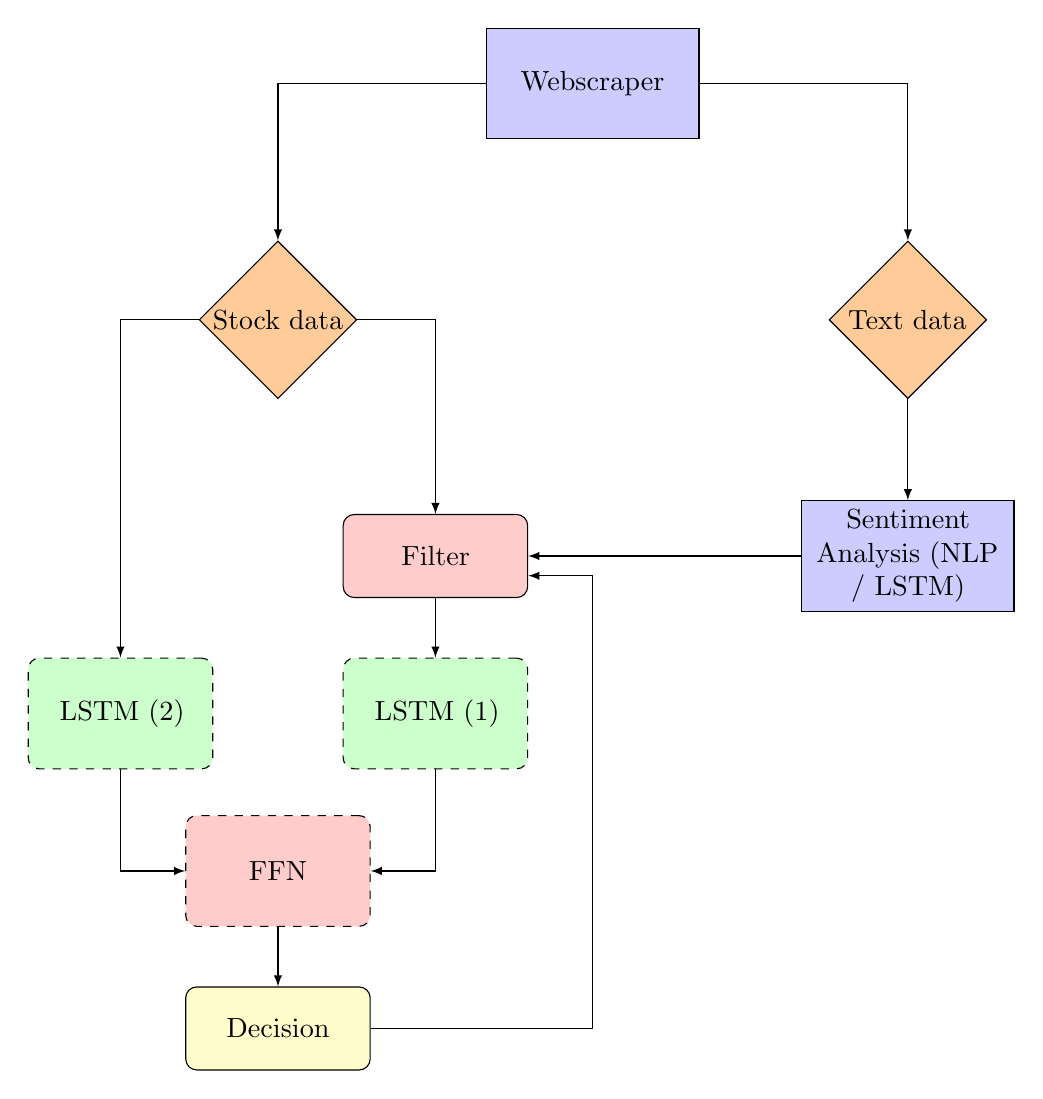
\begin{tikzpicture}[node distance = 2cm, auto]
      \tikzstyle{data} = [
        diamond,
        draw,
        fill=orange!40,
        text width = 5em,
        text badly centered,
        node distance = 3cm,
        inner sep = 0pt
      ]

      \tikzstyle{code} = [
        rectangle,
        draw,
        fill=blue!20,
        text width=7em,
        text centered,
        minimum height=4em
      ]

      \tikzstyle{network} = [
        rectangle,
        draw,
        dashed,
        fill=green!20,
        text width = 6em,
        text centered,
        rounded corners,
        minimum height = 4em
      ]

      \tikzstyle{feedforward} = [
        rectangle,
        draw,
        dashed,
        fill=red!20,
        text width = 6em,
        text centered,
        rounded corners,
        minimum height = 4em
      ]

      \tikzstyle{filter} = [
        draw,
        rectangle,
        fill=red!20,
        text width = 6em,
        text centered,
        minimum height=3em,
        rounded corners
      ]

      \tikzstyle{decision} = [
        draw,
        rectangle,
        fill=yellow!20,
        text width = 6em,
        text centered,
        minimum height=3em,
        rounded corners
      ]

      \node[code] (webscraper) at (0,6) {Webscraper};
      \node[data] (time series) at (-4,3) {Stock data};
      \node[data] (text) at (4,3) {Text data};
      \node[code] (processer) at (4,0) {Sentiment Analysis (NLP /
        LSTM)};
      \node[filter] (filter) at (-2,0) {Filter};
      \node[network] (lstm1) at (-2,-2) {LSTM (1)};
      \node[network] (lstm2) at (-6,-2) {LSTM (2)};
      \node[feedforward] (feedforward) at (-4,-4) {FFN};

      \node[decision] (decision) at (-4,-6) {Decision};

      \draw[-latex] (webscraper) -| (time series);
      \draw[-latex] (webscraper) -| (text);
      \draw[-latex] (text) -- (processer);
      \draw[-latex] (time series) -| (filter);
      \draw[-latex] (filter) -- (lstm1);
      \draw[-latex] (processer) -- (filter);
      \draw[-latex] (time series) -| (lstm2);
      \draw[-latex] (lstm2) |- (feedforward);
      \draw[-latex] (lstm1) |- (feedforward);
      \draw[-latex] (feedforward) -- (decision);
      \draw (decision) -- (0,-6) -- (0,-.25);
      \draw[-latex] (0,-.25) -- (-.82,-.25);
    \end{tikzpicture}
  \caption{Model overview}
  \label{fig:goal}
\end{figure}

\section{Classification}
Using LSTMs to predict stock pricing is, for the most part, a solved problem.
Implementations and hyperparameters may differ, of course, but underneath, the
structure of the model is largely the same. Hence, we decided to focus our work
on augmenting the filtering stage shown above. We wanted the network to have
access to both processed and unprocessed information,

\subsection{Frequency Analysis}

\end{document}
